\newpage
\section{Konzept}
Dieses Kapitel befasst sich mit der Ausarbeitung von drei möglichen Lösungskonzepten und deren Bewertung. Für die Auswahl der drei Lösungskonzepte wird die Methode des morphologischen Kastens nach Zwicky angewandt. In einer Tabelle werden alle gefunden Teillösungen nach Teilfunktion aufgelistet. Eine Gesamtlösung (Lösungskonzept) ergibt sich aus der Kombination von je einem Element pro Teilfunktion (Teillösung). Nach Neafe (2015) ist bei der selektiven Wahl der Elemente auf die Verträglichkeit der Elemente untereinander zu achten.
\newline
Die schiere Anzahl von möglichen Kombinationen ist ein Vorteil, kann jedoch auch überborden. Eine zu hohe Anzahl Kombinationen kann rasch zu einem Arbeitsaufwand führen, der nicht im gesetzten Zeitrahmen dieser Bachelorarbeit zu bewältigen wäre. Dieser Versuchung wird entgegnet indem sich die Auswahl auf drei Konzepte beschränkt. Weiter wird die Auswahl durch das Pflichtenheft eingeschränkt. Ungeeignete Kombinationen sind auszuschliessen, Kombinationen die den Fest- und Wunschanforderungen entsprechen sind zu bevorzugen.

Aus diesem Prozess sind drei Lösungskonzepte entstanden. Diese werden kurz vortstellt und einer Beurteilung unterzogen. Orientiert an der Beurteilung, steht am Ende der Konzeptphase der Entscheid, welches der drei Konzepte als Funktionsmuster umgesetzt wird.
\subsection{Lösungskonzepte}
Lösungskonzepte nur vorstellen, nicht bewerten.

\subsubsection{Konzept Grau}
Konzept Grau besteht aus drei Phasen:
\begin{itemize}
	\item \textbf{A - Vereinzelung mittels Schöpfrohrbunker:}
	Ein Schöpfrohrbunker dient zur Vereinzelung von Kugeln. Dabei werden NemaCaps in einem trichterförmigen Behälter (Punkt 2 in Abbildung XY) gesammelt. Zu unterst im Trichter befindet sich ein Rohr (1), welches eine Translation ausübt. Durch die Translation wird das unterste Gefüge so bewegt, dass ein oder mehrere NemaCaps ins Rohr fallen. So werden die NemaCaps in einer Reihe geordnet.
	
	\item \textbf{B - Auslösen und Transport mittels Pneumatik:}
	Aufeinander gestapelt, werden die NemaCaps von der Auslösung abgefertigt. Dabei wird das unterste NemaCaps mit einer linearen Bewegung (3) zu einer Öffnung geschoben. Zusätzlich wird das NemaCap an der Öffnung durch ein Vakum angesaugt. Durch einen Schlauch wird das NemaCap mittels Pneumatik zur Einsetzlokalität transportiert. 
	
	\item \textbf{C - Setzen mittels Rohr:}
	Zeitgleich zu Phase A und B wird am Topf das Setzen der NemaCaps vorbereitet. Dafür wird ein Rohr (4) in den stehenden Topf bis zur Setztiefe eingetaucht. Ist dieser eingetaucht, wird das NemaCap durch die Pneumatik zum Rohrende transportiert und somit im Topf platziert. Das Rohr fährt aus dem Topf, der Prozess beginnt von vorne.
\end{itemize}

Die Konfiguration des Setzmechanismus wird dabei durch die radiale Verstellung der einstechenden Rohre gewährleistet. Hierfür ist die manuelle Einstellung des Rohrs in radialer Richtung notwendig und vor jedem Batch auszuführen.

Dabei muss gewährleistet sein, dass das eintauchende Rohr nicht durch Erdpartikel verstopft wird.
\begin{figure}[H]
	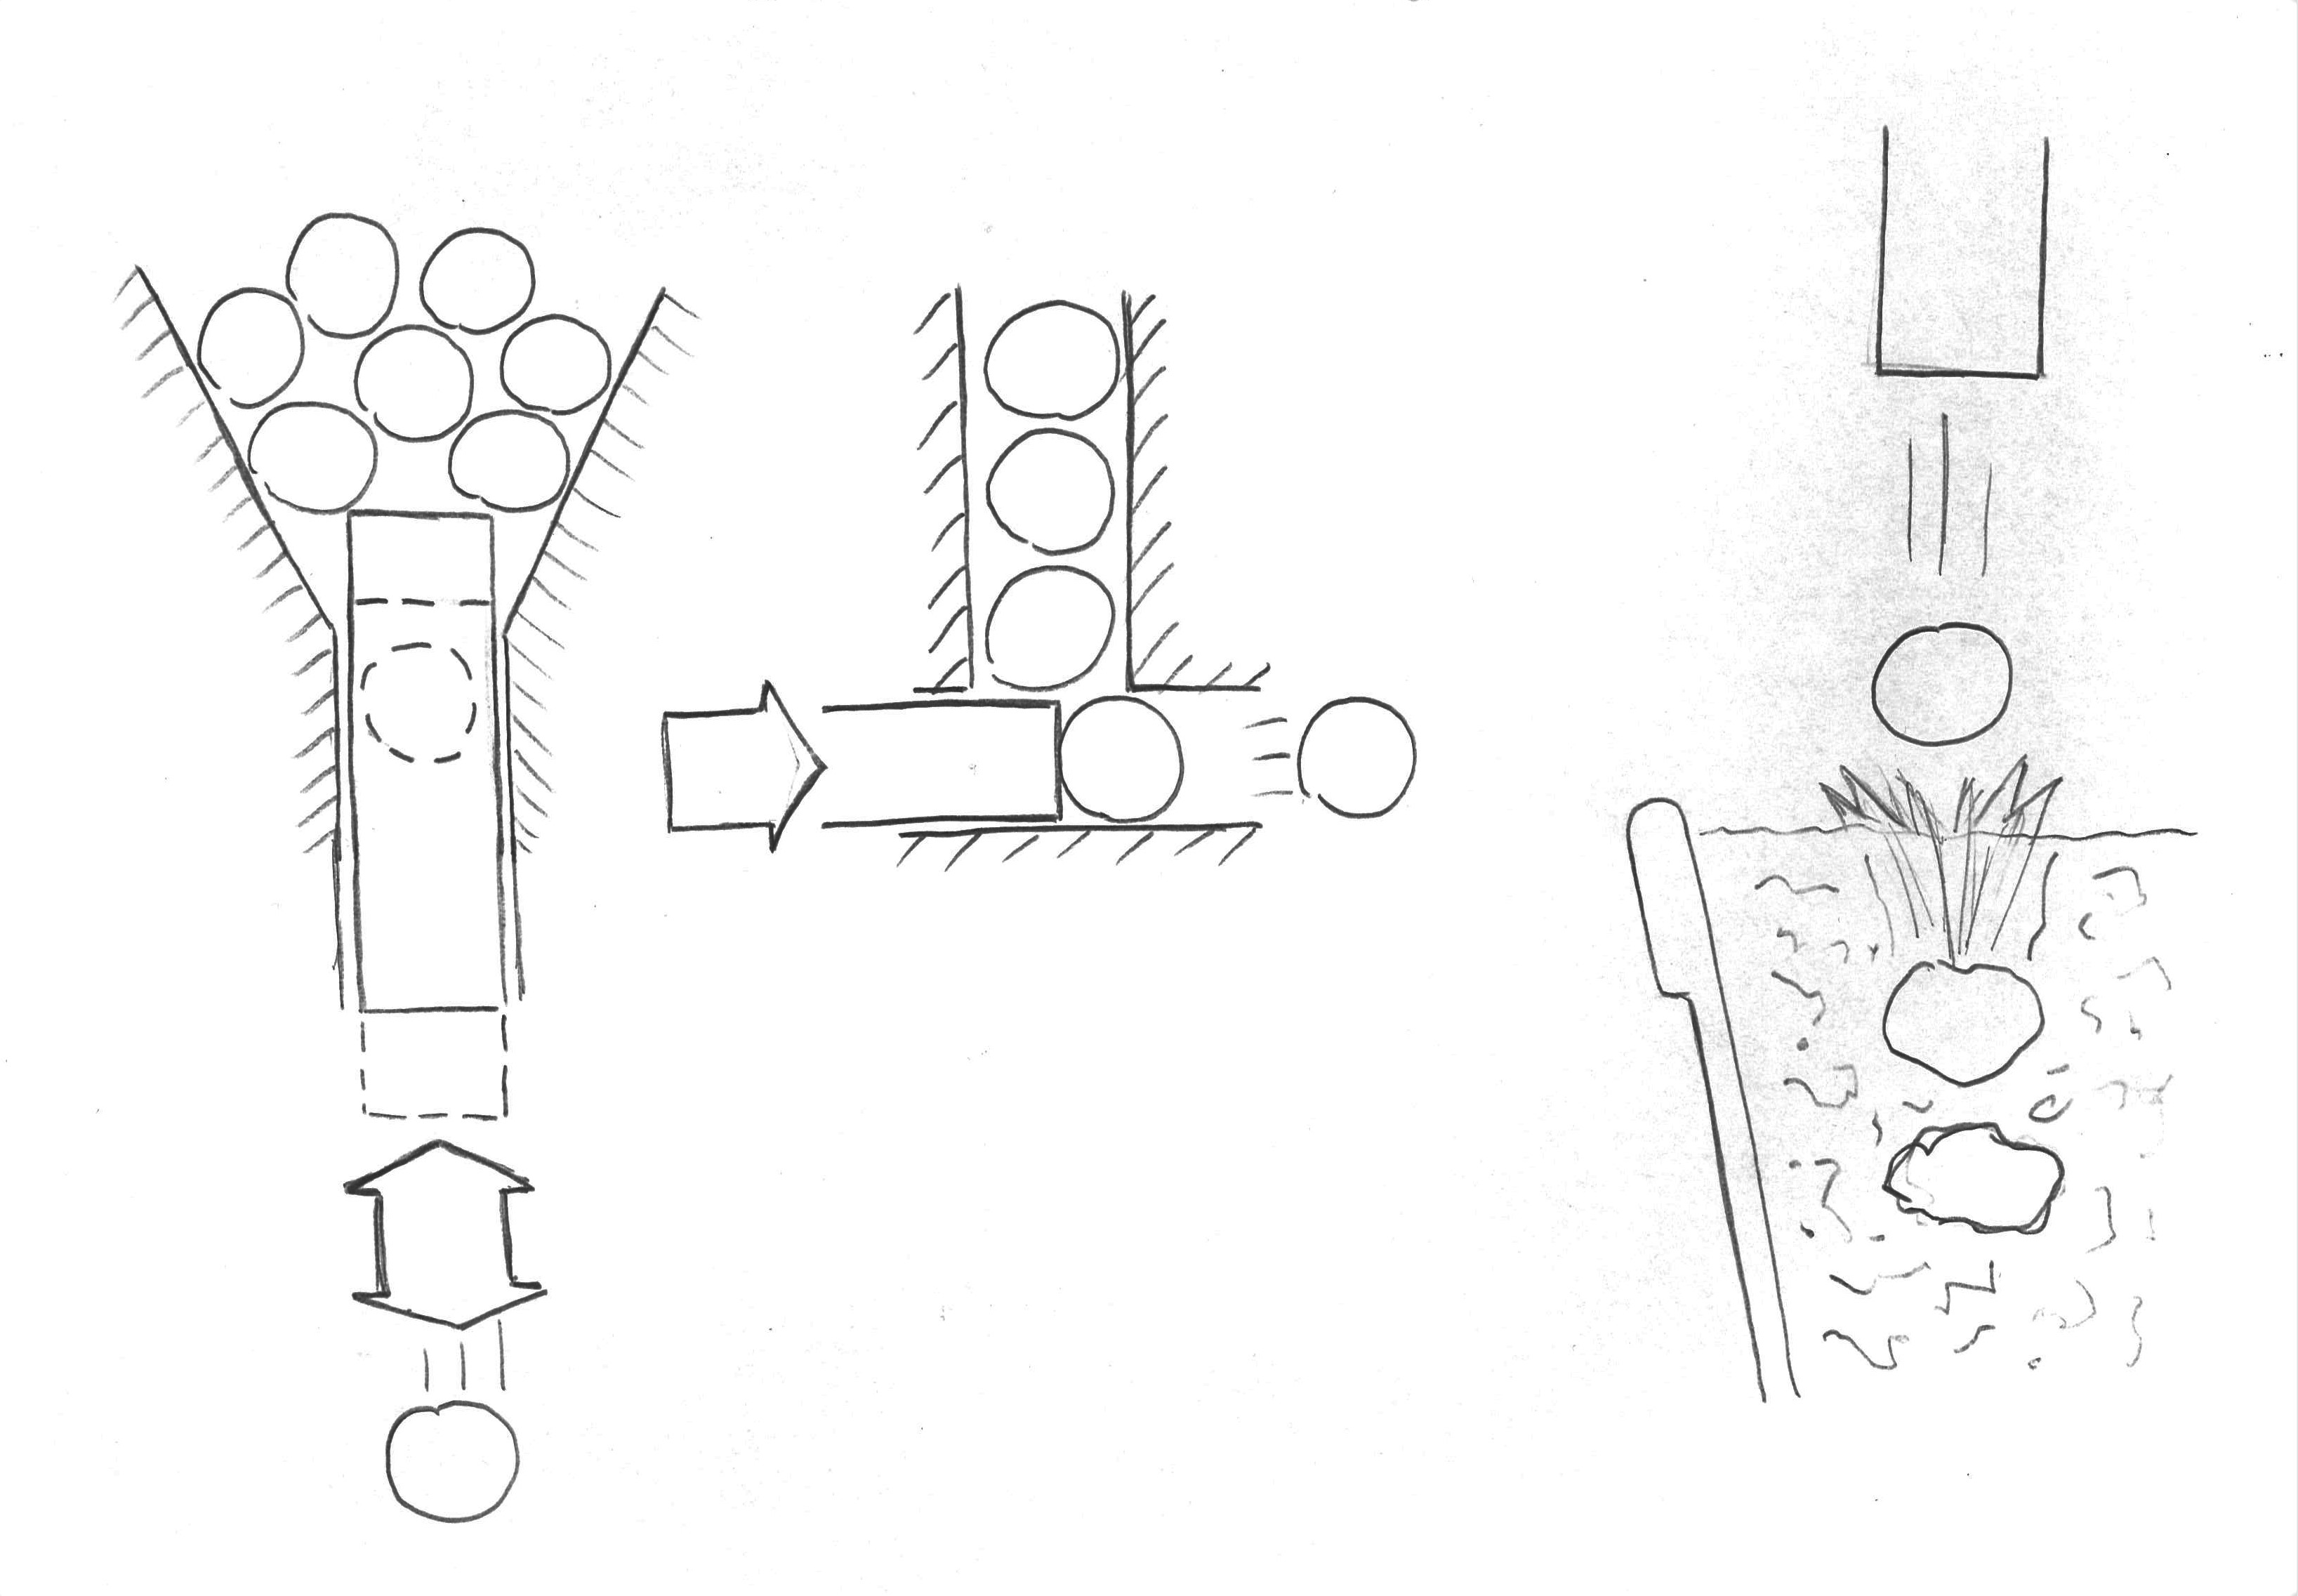
\includegraphics[scale=0.6]{Illustrationen/5-Konzept/grau_Konzept.jpg}
	\caption{Konzeptskizze von Konzept Grau}
	\label{fig:konzept_grau}
\end{figure}

\subsubsection{Konzept Grün}
\label{KonzeptGreen}
Konzept Grün besteht aus diesen Teillösungen:
\newline

\textbf{Vereinzelung durch Wendelförderer}
\begin{wrapfigure}[13]{r}{7.5cm}
	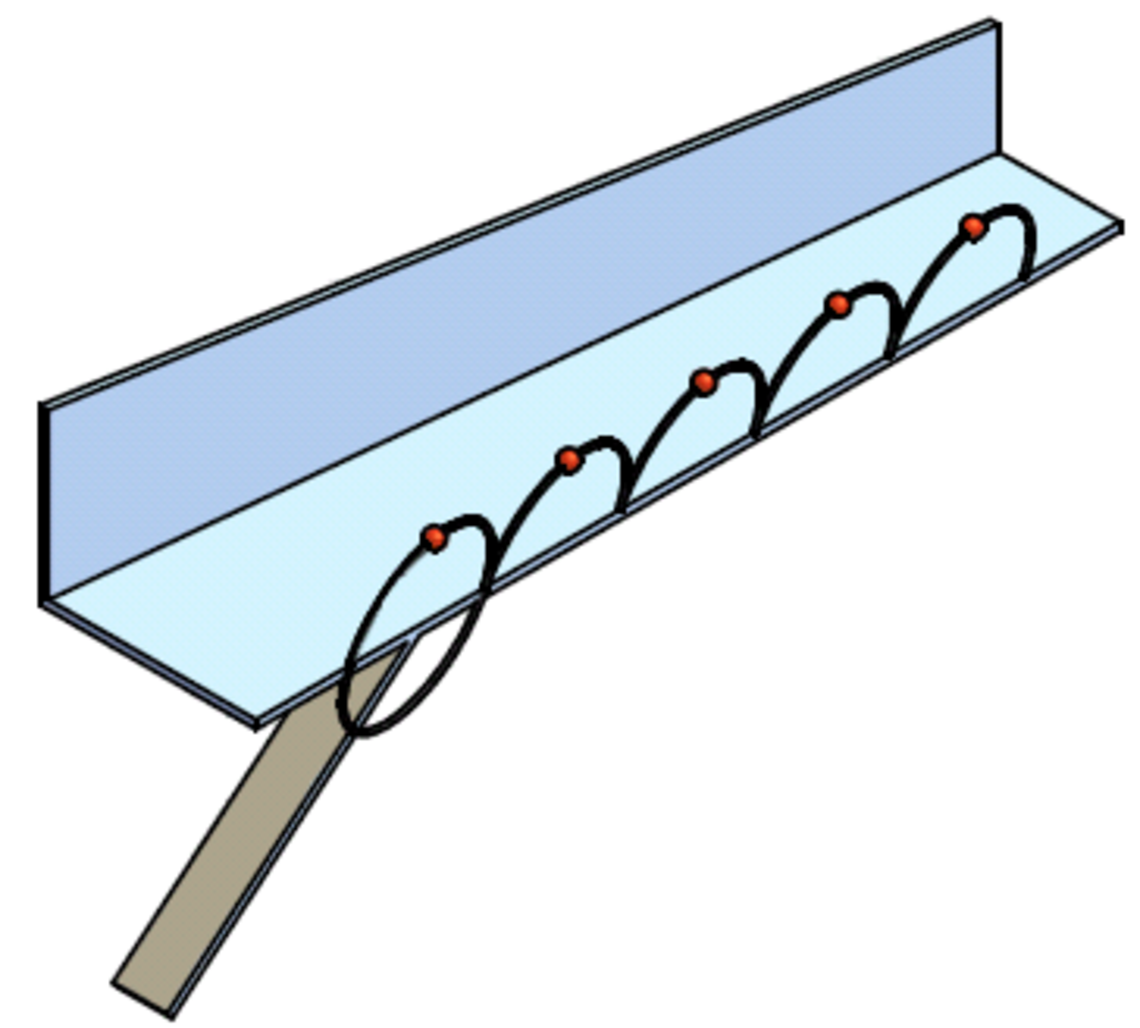
\includegraphics[scale=0.2]{Illustrationen/5-Konzept/foerderbewegung.png}
	\caption{Wurfbewegung erzeugt durch Vibration}
	\label{fig:foerderbewegung}
\end{wrapfigure}
\begin{wrapfigure}[14]{r}{7.5cm}
	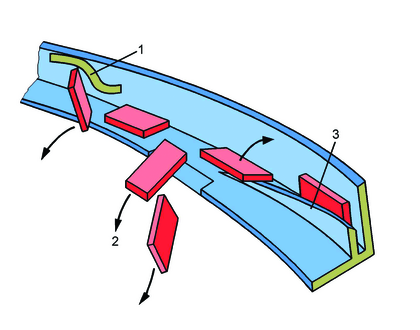
\includegraphics[scale=2.0]{Illustrationen/5-Konzept/schikane.png}
	\caption{Vereinzelung durch Schikanen}
	\label{fig:schikane}
\end{wrapfigure}
Das Konzept Grün beinhaltet die Verzeinzelung sowie Förderung von NemaCaps mit einem Vibrationswendelförderer (siehe Abbildung \ref{fig:vereinzelung_green}). Vibration ist für die Vereinzelung sowie Förderung von Gütern mit einfacher Geometrie oft genutzte Technik. Dabei wird nach Webac GmbH (2017) mittels Schwingungsenergie (erzeugt durch eine Unwuchterregung mittels Vibrator) die zu bewegende Masse erregt und eine Hin- und Rückbewegung erzeugt. Dabei wird die Masse so angestossen, dass eine Kette von Wurfbewegungen entsteht und sich die Masse fortbewegt (siehe Abbildung \ref{fig:foerderbewegung}).
\newline

Die Vereinzelung wird mit Schikanen realisiert. Diese gewährleisten durch Abstimmung der Werkstückkontur, dass jeweils nur ein Werkstück die Schikane passiert und weiter gefördert wird (siehe Abbildung \ref{fig:schikane}). Überzählige werden zurück ins Haufwerk gelenkt (Handling online, 2006).
\newline
Der vorgesehene Wendelförderer basiert auf den erwähnten Techniken. In einer Spirale werden durch die Vibration die Werkstücke gefördert und sogleich vereinzelt. Speziell an dieser Anwendung ist, dass die NemaCaps in drei parallele Bahnen geteilt werden. Auch denkbar ist die Verwendung von drei einzelnen Wendelförderer.
\newline
\begin{figure}[H]
	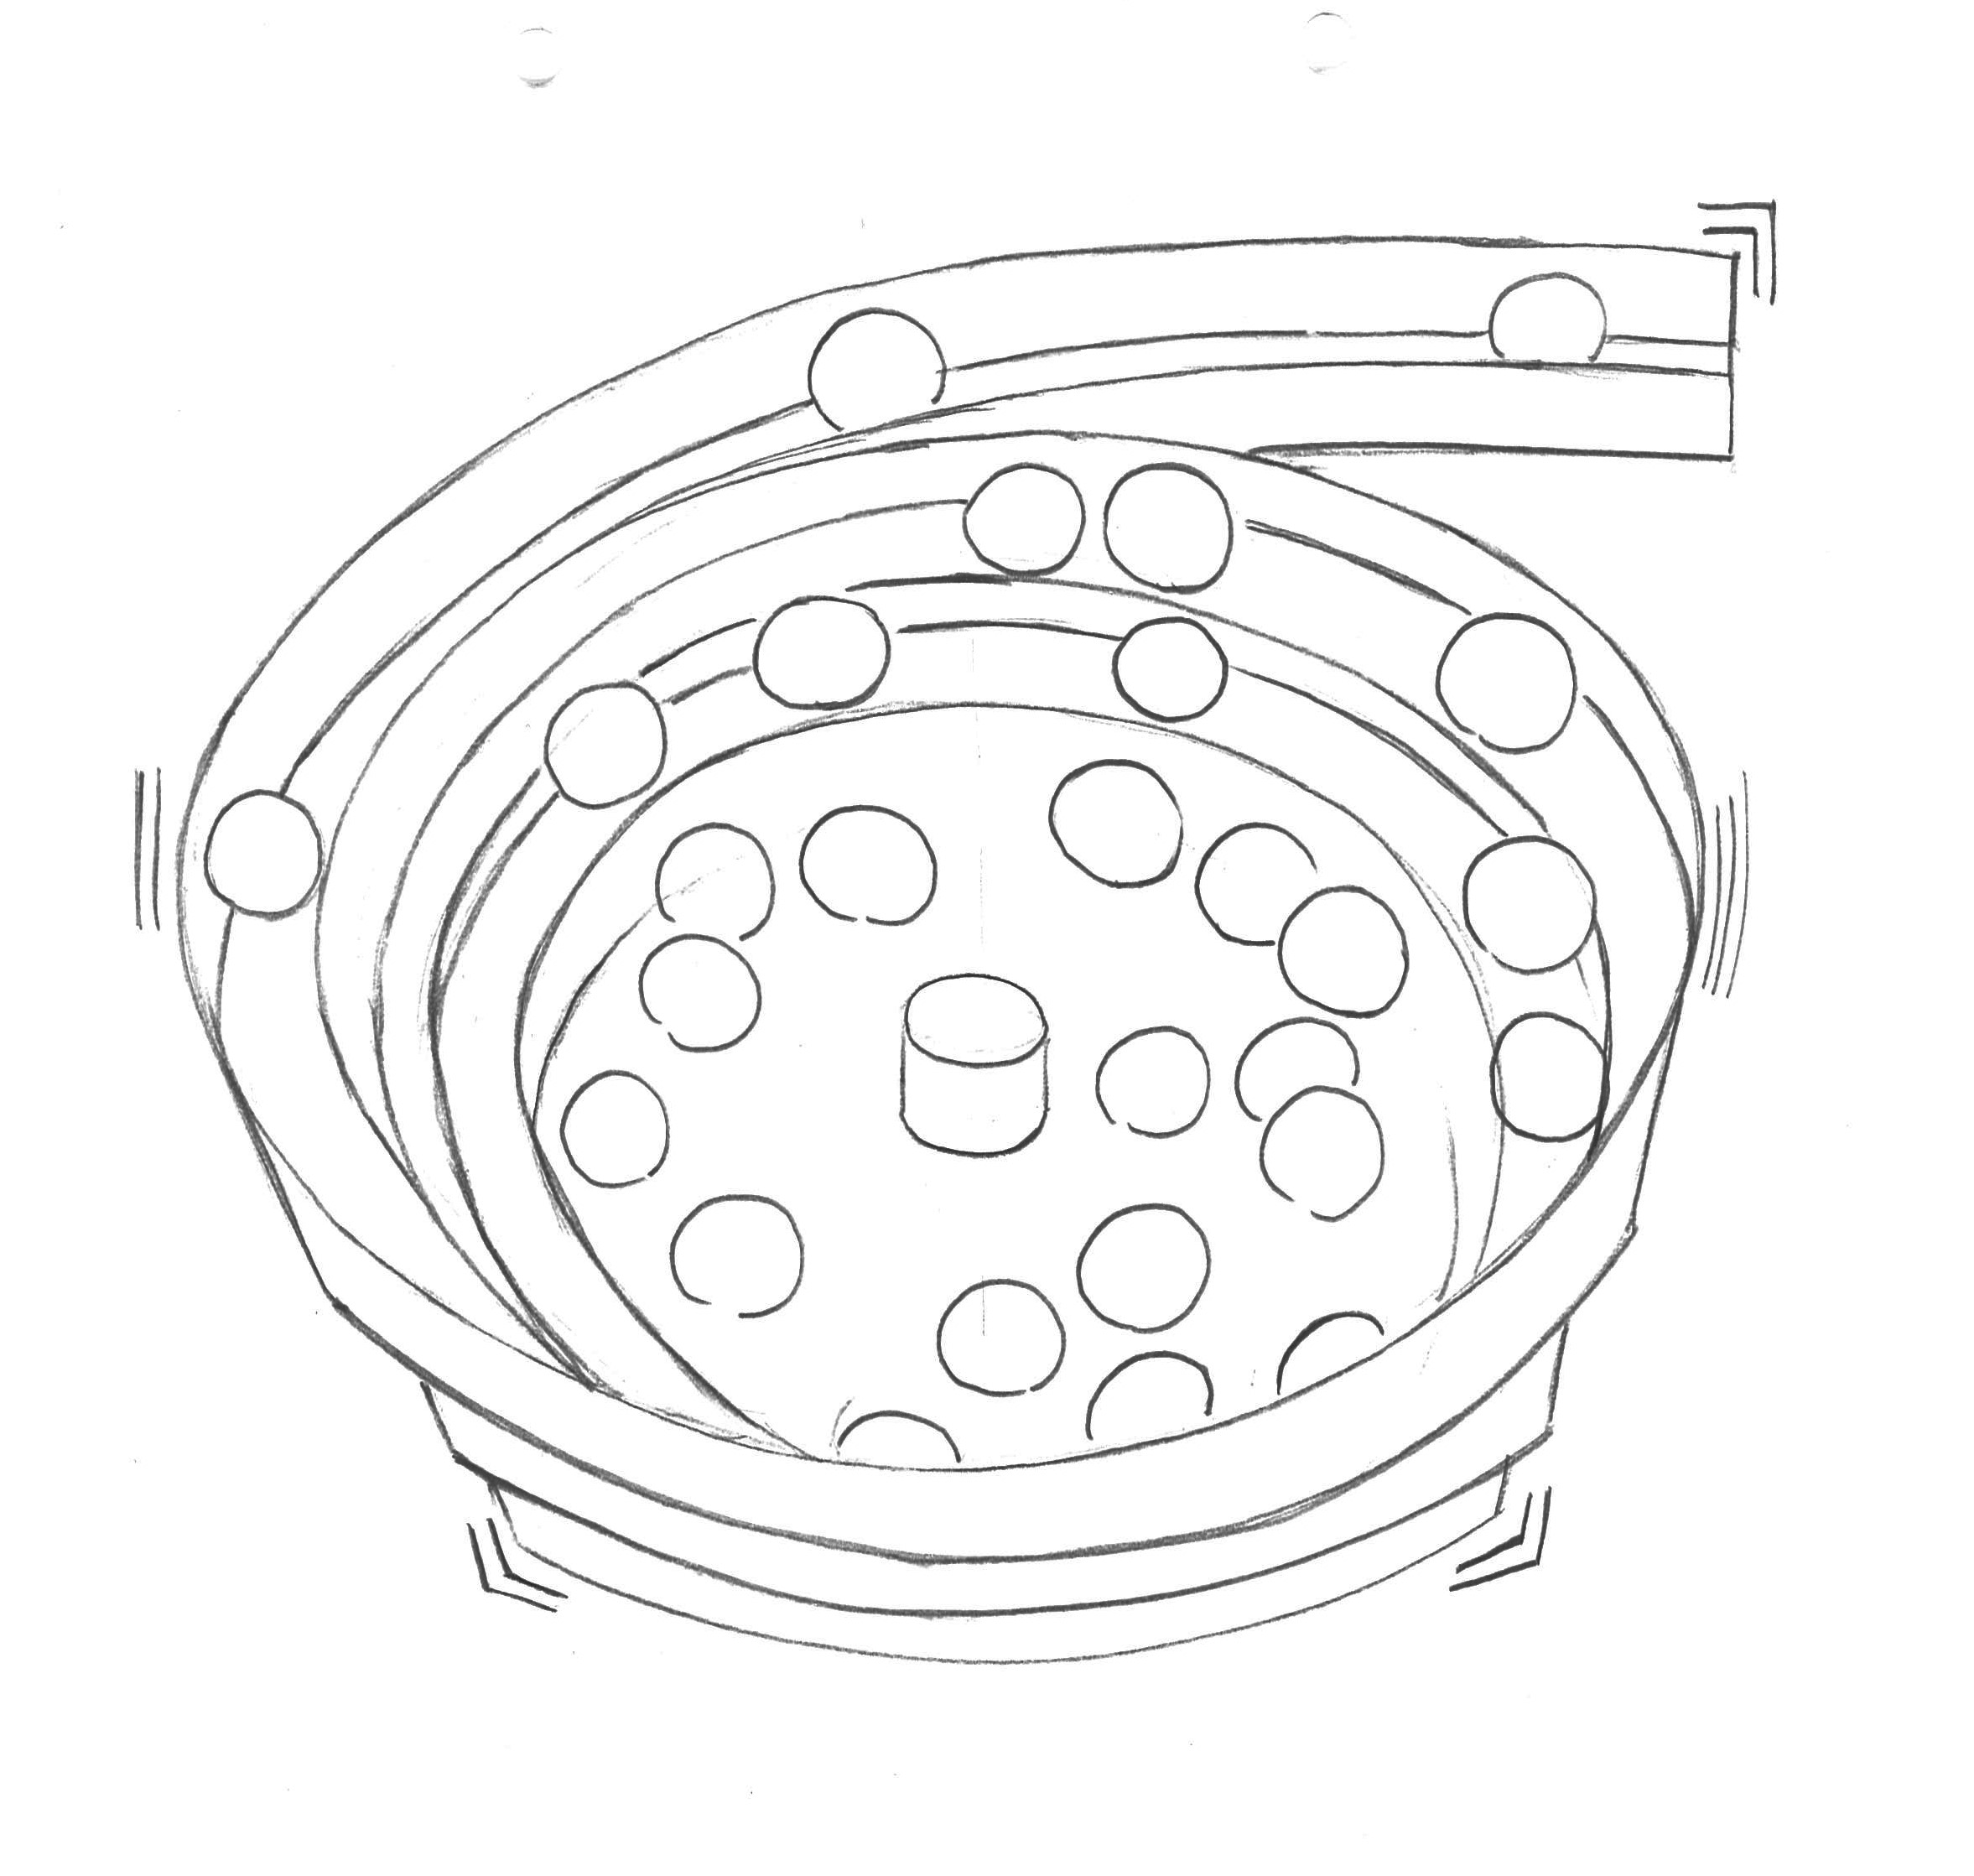
\includegraphics[scale=0.6]{Illustrationen/5-Konzept/green_wendelfoerderer.jpg}
	\caption{Konzeptskizze I Konzept Grün: Wendelförderer}
	\label{fig:vereinzelung_green}
\end{figure}

\textbf{Setzen mittels Pick-and-Place Bewegung}
\newline
Die NemaCaps kommen geordnet bei der Setzeinheit an. Dabei werden diese an einem mechanischen Anschlag gestoppt (Siehe Punkt 1 in Abbildung XY). Von dort werden die NemaCaps durch eine Setzeinheit gepackt und in den Töpfen platziert. Dabei ist die Setzeinheit als zweidimensionale Pick-and-Place Maschine aufgebaut. Diese zwei Dimensionen sind:
\begin{itemize}
	\item Translation in X-Richtung: Diese Bewegung dient zum horizontalen Transport von mechanischem Anschlag zum Topf.
	\item Translation in Z-Richtung: Um das NemaCap zu Packen sowie im Topf zu platzieren wird diese Bewegung ausgeführt.
\end{itemize}
Zur Übersicht dient Abbildung \ref{fig:transport_green_pers}. 
\begin{figure}[H]
	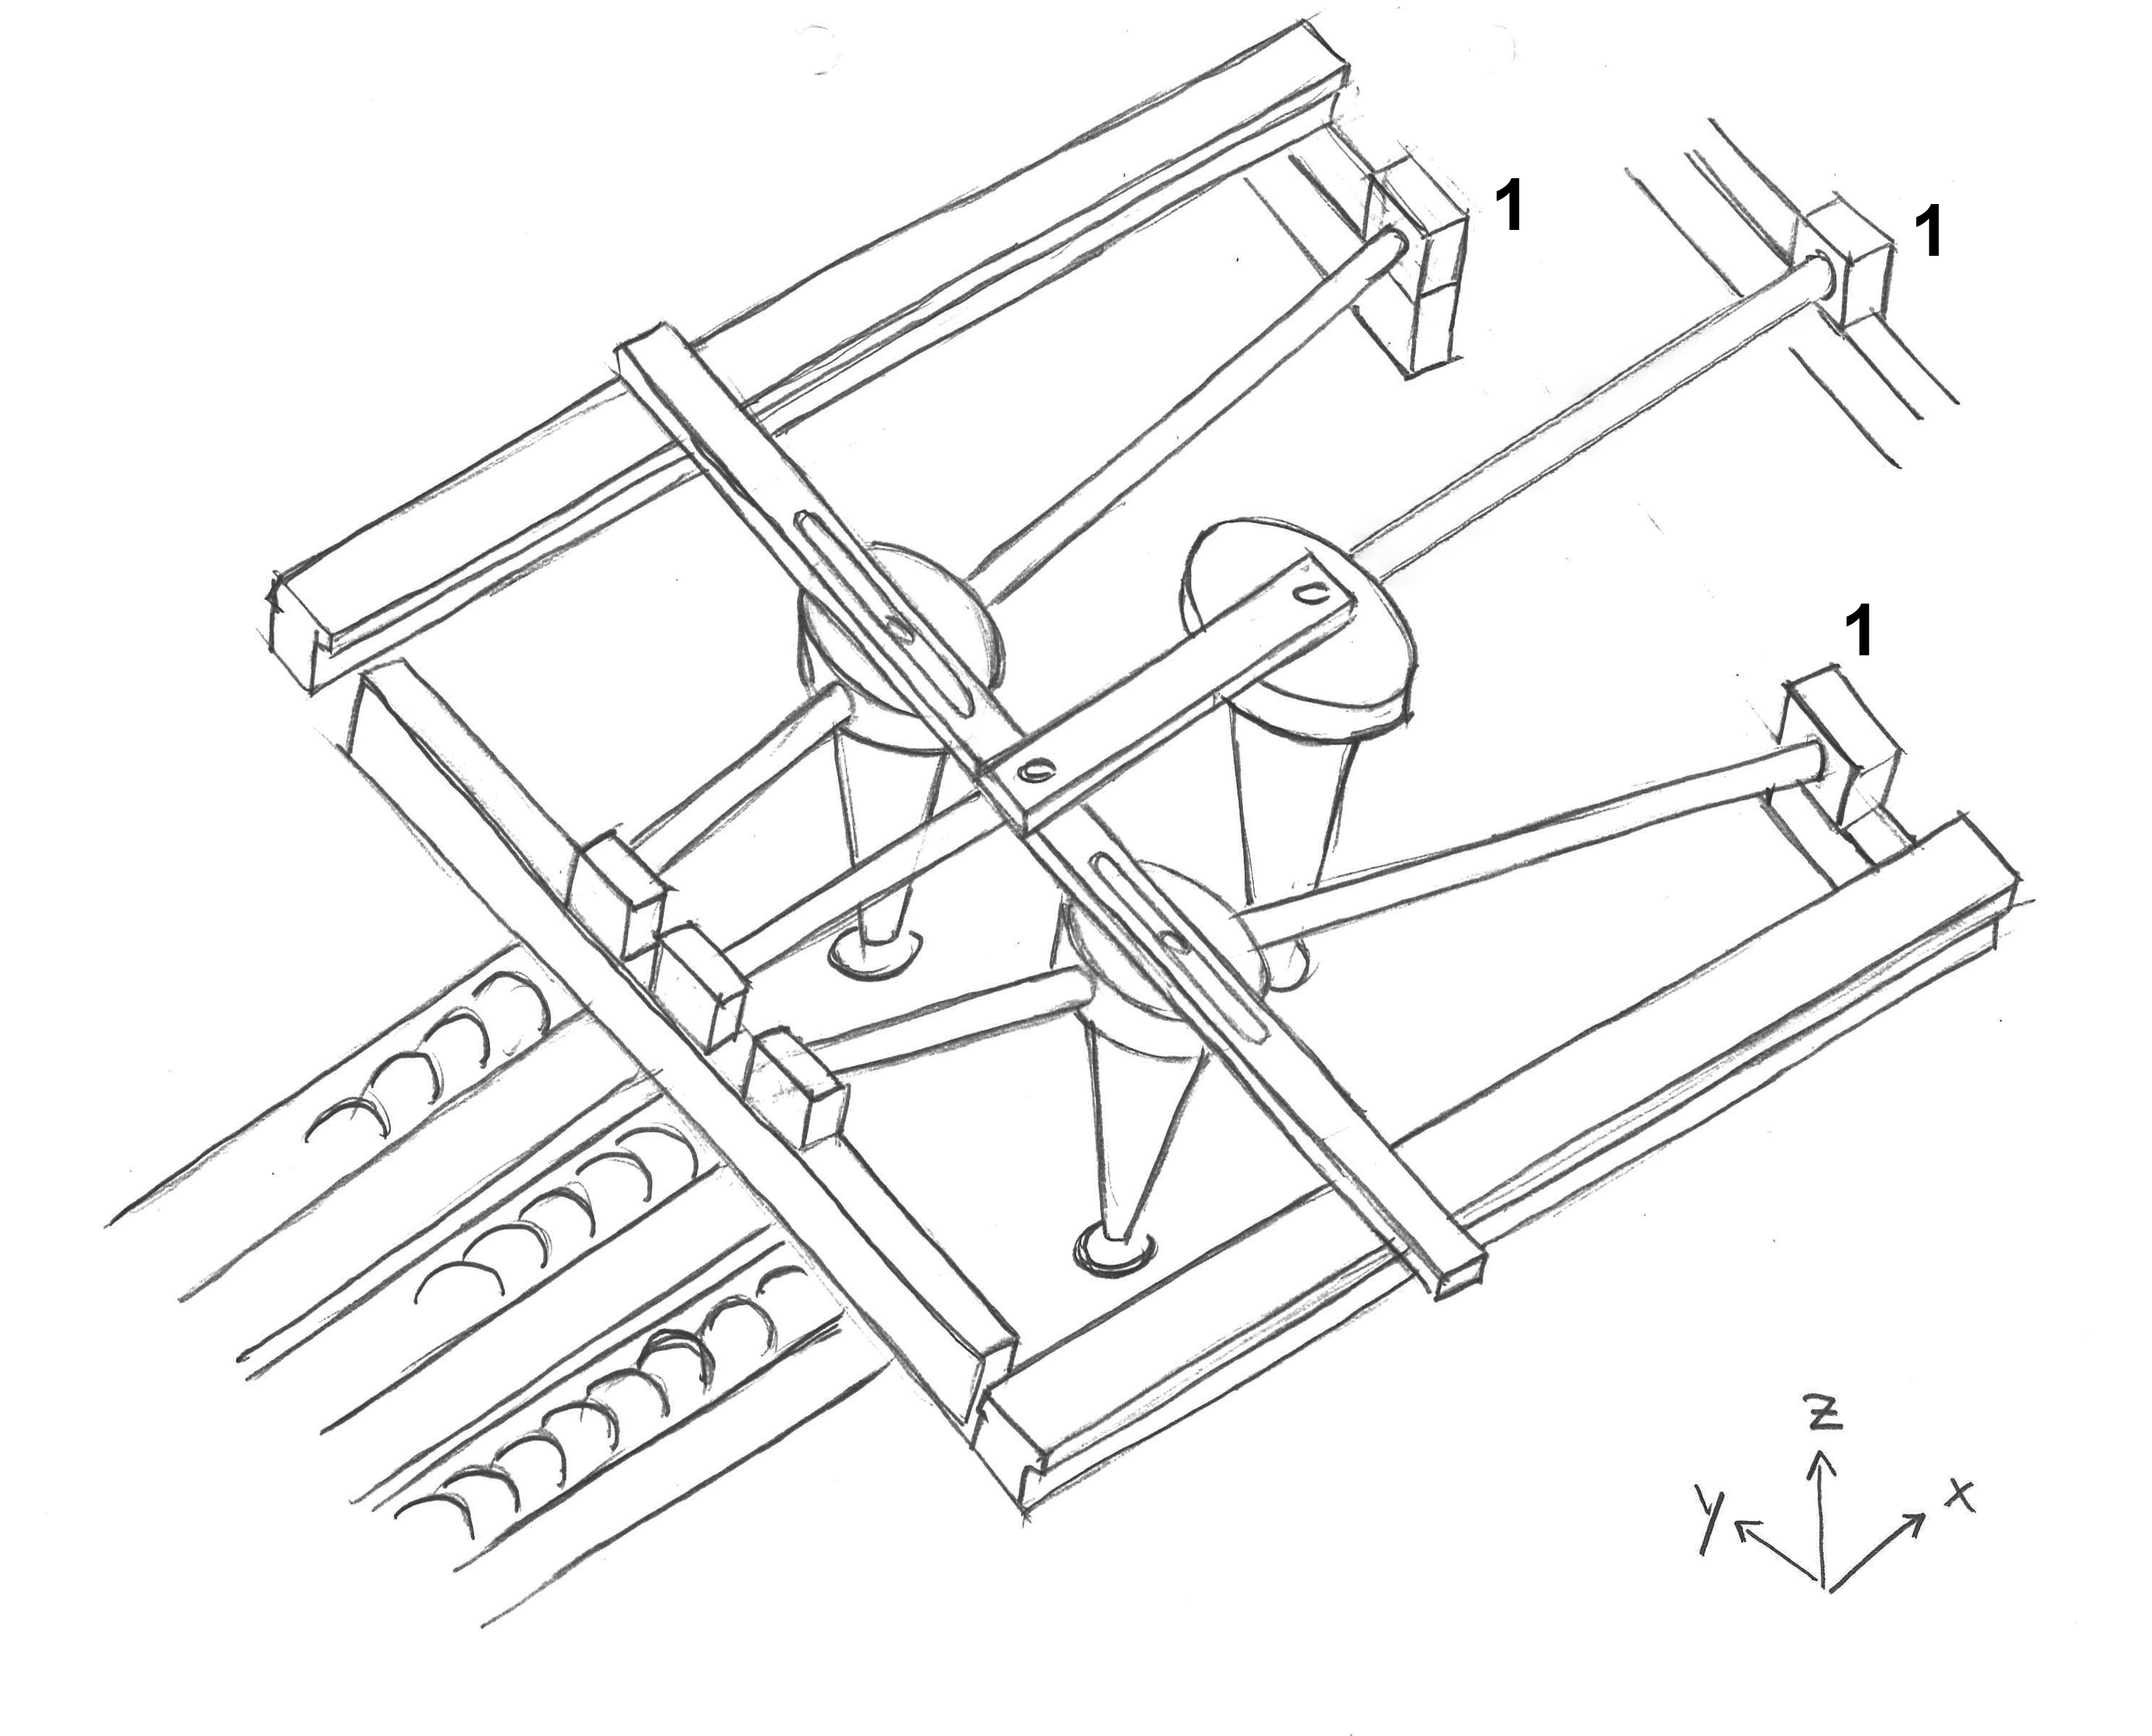
\includegraphics[scale=0.6]{Illustrationen/5-Konzept/green_2Dmachine_pervsp.jpg}
	\caption{Konzeptskizze II Konzept Grün: Perspektivische Ansicht der Pick-and-Place Bewegung}
	\label{fig:transport_green_pers}
\end{figure}

Der Prozess der Setzeinheit gestaltet sich folgendermassen:
\begin{itemize}
	\item \textbf{A - NemaCap packen:} Sobald der bewegte Teil der Seitzeinheit sich über dem NemaCap befindet, packen drei Dorne je ein NemaCap (Detail A in Abbildung XY). Für das Packen sind folgende Techniken möglich:
	\begin{itemize}
		\item Mittels Zange wird das NemaCap seitlich gefasst.
		\item Durch einen spitzen Dorn wird das NemaCap aufgespiesst (Gemäss Pflichtenheft zulässig).
		\item Durch einen stumpfen Dorn mit hoher Adhäsion (zum Beispiel Kleber) wird das NemaCap angeheftet.
		\item Mittels Unterdruck wird das NemaCap an eingem Dorn angesaugt.
	\end{itemize} 
	\item \textbf{B - NemaCap transportieren:} Das NemaCap wird durch die Bewegung in X-Richtung über die Einsatzlokalität transportiert. Dabei werden die einzelnen Dorne durch Laufschienen geleitet und so auf den entprechenden Topfradius gelenkt. Die einzelnen Dorne sind miteinander verbunden, sodass diese lineare Bewegung nur ein Aktor erfordert.
	\item \textbf{A - NemaCap setzen:} 
	Über der Einsetzlokalität angekommen, bewegt sich der Dorn in Z-Richtung nach unten und stösst das NemaCap in die Erde. Dabei wird eine Beschädigung des NemaCaps bewusst in Kauf genommen, da dies gemäss Pflichtenheft zulässig ist. Wichtig ist, dass beim Zurückfahren des Dorns sich das NemaCap vom Dorn löst.
\end{itemize}
Die Konfiguration des Setzmechanismus ist durch die Verstellung der Laufschienen möglich. Dabei sind die Laufschienen am oberen Ende (über dem Topf) in Y-Richtung verstellbar. So können die verschiedenen Topfgrössen gehandhabt werden.

\begin{figure}[H]
	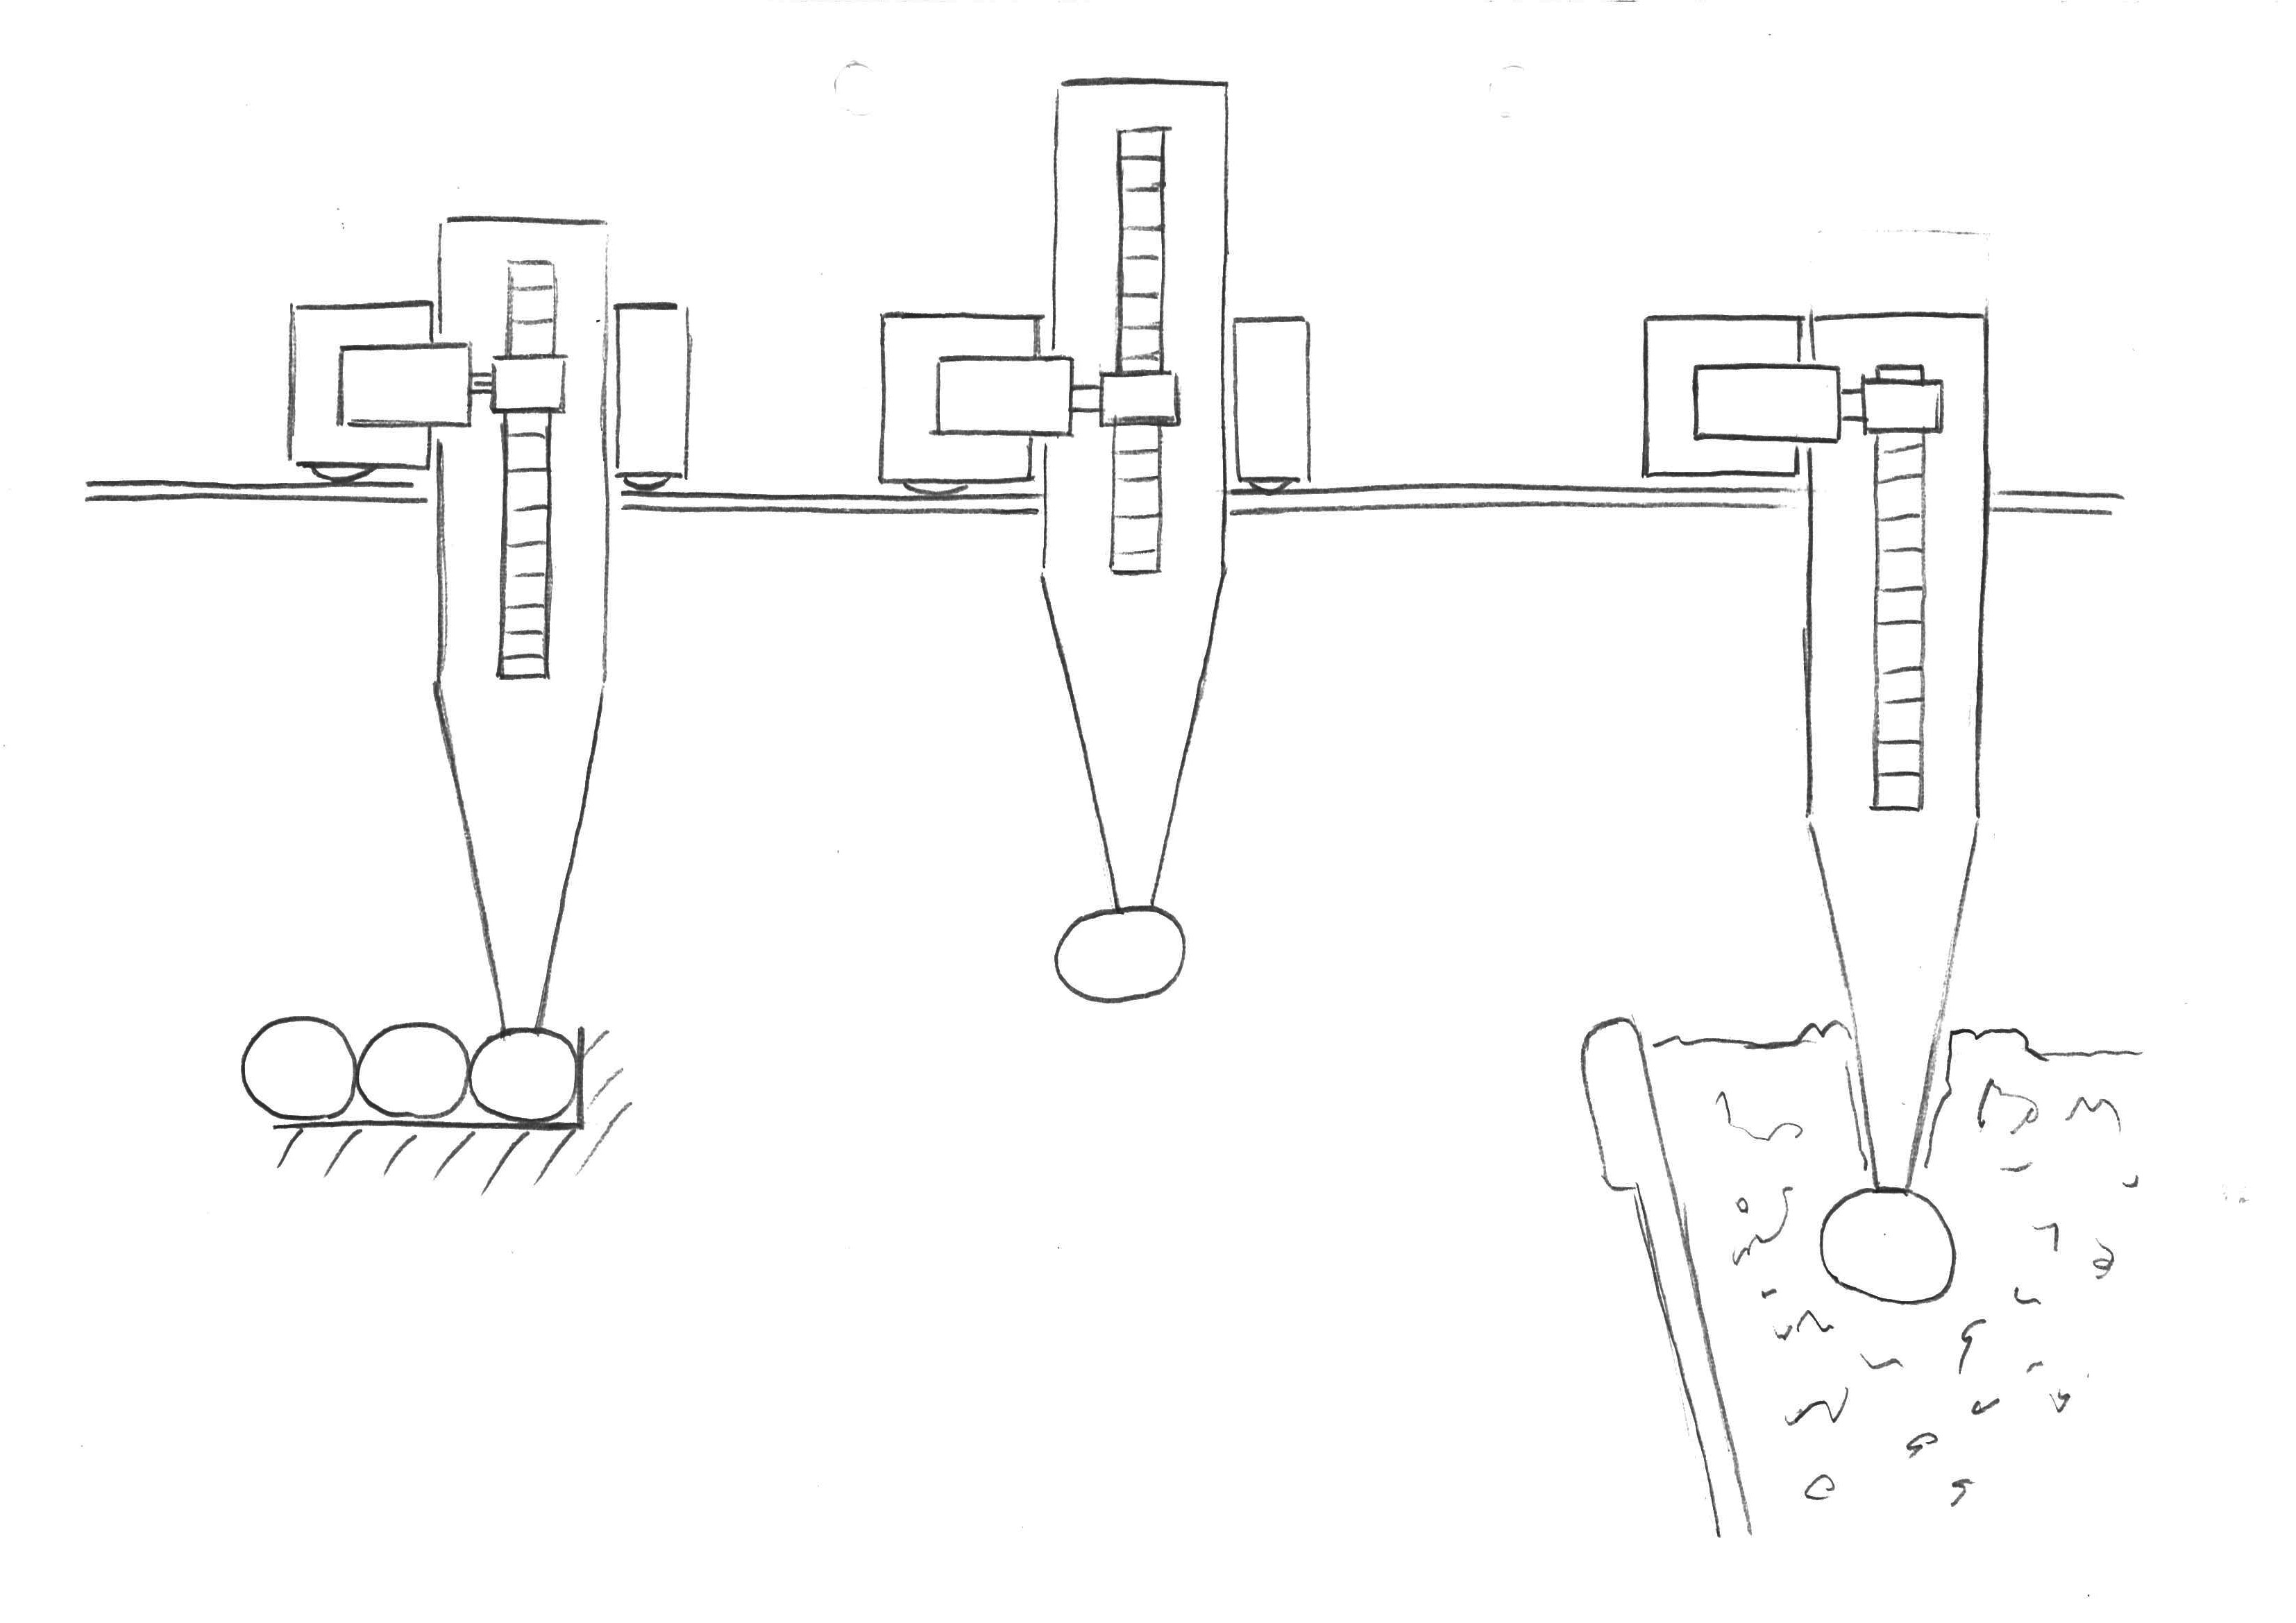
\includegraphics[scale=0.6]{Illustrationen/5-Konzept/green_2Dmachine_seite.jpg}
	\caption{Konzeptskizze III Konzept Grün: Seitenansicht der Pick-and-Place Bewegung}
	\label{fig:transport_green_side}
\end{figure}
\subsubsection{Konzept Blau}